
\documentclass[11pt,a4j]{jreport}
\renewcommand{\baselinestretch}{1.4}
\usepackage{comment}
\usepackage{float}
\usepackage{color}
\usepackage{multicol}
%\usepackage[dvipdfmx]{pict2e}
\usepackage{wrapfig}
%\usepackage{graphicx}
\usepackage[dvipdfmx]{graphicx}
\usepackage{bm}
\usepackage{url}
\usepackage{underscore}
\usepackage{colortbl}
\usepackage{tabularx}
\usepackage{fancyhdr}
\usepackage{ulem}
\usepackage{cite}
\usepackage{amsmath,amssymb,amsfonts}
\usepackage{algorithmic}
\usepackage{textcomp}
\usepackage{xcolor}
\usepackage{booktabs}
\usepackage{longtable}
\usepackage[ipaex]{pxchfon}

\usepackage{listings,jvlisting}
\lstset{
  basicstyle={\ttfamily},
  identifierstyle={\small},
  commentstyle={\smallitshape},
  keywordstyle={\small\bfseries},
  ndkeywordstyle={\small},
  stringstyle={\small\ttfamily},
  frame={tb},
  breaklines=true,
  columns=[l]{fullflexible},
  numbers=left,
  xrightmargin=0zw,
  xleftmargin=3zw,
  numberstyle={\scriptsize},
  stepnumber=1,
  numbersep=1zw,
  lineskip=-0.5ex
}
\renewcommand{\lstlistingname}{プログラム}

\usepackage[top=30truemm,bottom=30truemm,left=30truemm,right=30truemm]{geometry}

\begin{document}

\thispagestyle{empty}
\begin{center}
\
\vspace{3cm}

{\huge{Vitis Vision Libraryを用いた画像処理の\\
ハードウェア実装と性能評価}}

\vspace{9mm}

{\LARGE 指導教員}

\vspace{5mm}

{\LARGE 高橋 寛 教授}

\vspace{4mm}

{\LARGE 甲斐 博 准教授}

\vspace{4mm}

{\LARGE 王森レイ 講師}

\vspace{20mm}

{\LARGE 令和 5 年 1 月 20 日提出}\\

\vspace{20mm}

{\LARGE 愛媛大学工学部工学科}\\

\vspace{4mm}

{\LARGE 応用情報工学コース}\\

\vspace{4mm}

{\LARGE 計算機/ソフトウェアシステム研究室}\\

\vspace{18mm}

{\huge 西川 竜矢}\\

\end{center}

\thispagestyle{empty}
\clearpage

% 目次の表示
\tableofcontents

%=====================================================================================
\pagestyle{fancy}
\lhead{\rightmark}
\renewcommand{\chaptermark}[1]{\markboth{第\ \normalfont\thechapter\ 章~~#1}{}}
%=====================================================================================
%
%========序論=========================================================================
\chapter{序論} %章

\section{研究背景}

近年,日常生活を送るうえで多くの場面でIoTが活用されている.また,エッジAIの登場により,
IoT機器における処理全体に要する時間の短縮に成功している.その中でも,自動車の歩行者検知や
製造業における外観検査などに使われている技術に物体検出がある.物体検出には高いリアルタイム性
が求められているが,IoT機器におけるエッジデバイスは推論モデルの学習環境に用いられるPCと比較すると
CPU性能やメモリ容量といったリソースが劣る.こうした現状から,限られたリソースの中で,
処理速度やリソース使用量などのパフォーマンスをどれだけ向上させられるかが課題となっている.

物体検出の流れとしてはじめに入力画像に対する前処理を行い,ここで整形された画像データを用いて
推論処理を行う.これらの工程において,入力画像に対する前処理よりも,推論処理の方が処理に要する
時間が大きくなる.そのため,前処理に対する高速化の研究よりも推論処理に対する高速化の研究の方が
盛んである.推論処理に対する高速化手法\cite{AccelTemp}は,主流な方法である量子化をはじめ,
レイヤフュージョン,デバイス最適化,マルチスレッド化などさまざまである.
今後さらに推論処理の高速化が進んでくると,高速化された推論処理に対して,その前に処理速度の遅い前処理の工程が
入ってくるため,折角高速化した推論処理のパフォーマンスを最大限に発揮できなくなってしまう恐れがある.

加えて,エッジコンピューティングにおいて注目すべきはそのエッジデバイスである.
FPGA(Field Programmable Gate Array)は,コンピュータをはじめ通信機器やプリンタなど多くのエッジデバイスに搭載され用いられている.
その大きな特徴として現場で論理回路の構成を書き換え可能である点が挙げられる.
また,FPGAは大量のデータを高速に処理し,さらに消費電力が低いという利点がある.
%以上の点から,リアルタイム性を重要視している
%エッジデバイスでの画像処理に対してFPGAを用いることは,先に述べた課題に対する有効的な解決策となるといえる.

以上の点から,本研究では,物体検出におけるリアルタイム性を課題として取り上げ,入力画像に対する前処理を
高速化することを目的とする.目的達成のための方法としてFPGAを用いたハードウェアアクセラレーションを用いる.
高速化した前処理と,そうでない前処理に対して処理速度の計測を行い,ハードウェアアクセラレーションによりどの程度
処理時間を短縮できたかを検証する.

\section{論文の構成}
※全体が完成したら書きます.
%本論文ではエッジコンピューティングにおける物体検出の入力画像に対する前処理の高速化について
%本論文の構成について述べる.第1章では研究背景について述べる.第2章では本論文を読むにあたって必要となる予備知識
%について,画像処理およびFPGAの観点から説明する.第3章では本研究で扱う画像処理アプリケーションの実装について,
%開発環境,開発フロー及び
%
%========予備知識=========================================================================
\chapter{準備}
本章では,この論文を読むにあたって理解しておく必要のある予備知識について述べる.
\section{画像処理}
\subsection{物体検出}
機械学習を活用して画像に映る特定の物体を検出する技術を物体検出と呼ぶ.
物体検出における大まかな流れを図2.1に示す.
\begin{figure}[H]
  \center
  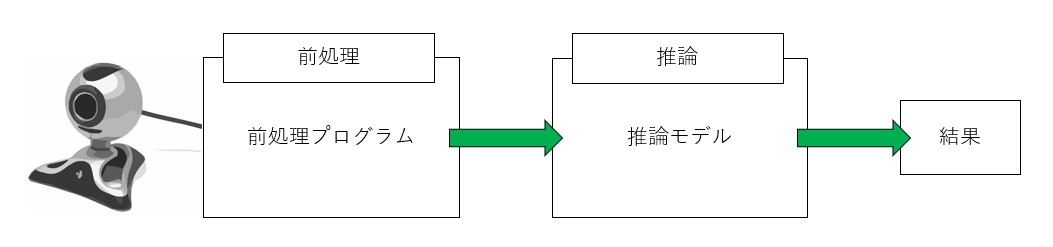
\includegraphics[scale = 0.8]{pict/pict4.jpg}
  \caption{物体検出の流れ}
\end{figure}
物体検出の流れとして,はじめにカメラから入力画像を取得する.
この画像に対して画像前処理を行う.この処理は画像データの整形を行い,整形したデータを
推論モデルに渡す.
整形された画像データを受け取った推論モデルは推論処理を行い,
推論結果を出力する.こうした流れで物体検出技術は実現されており,
製造業や自動車分野,さらには医療分野など幅広い分野で利用されている.

\subsection{物体検出の詳細}
本研究における物体検出の詳細について示す.
本研究では推論モデルに,YOLOv3 tinyおよびYOLOv4を想定しており,
入力画像に対する前処理はリサイズを行う.
\begin{figure}[H]
  \center
  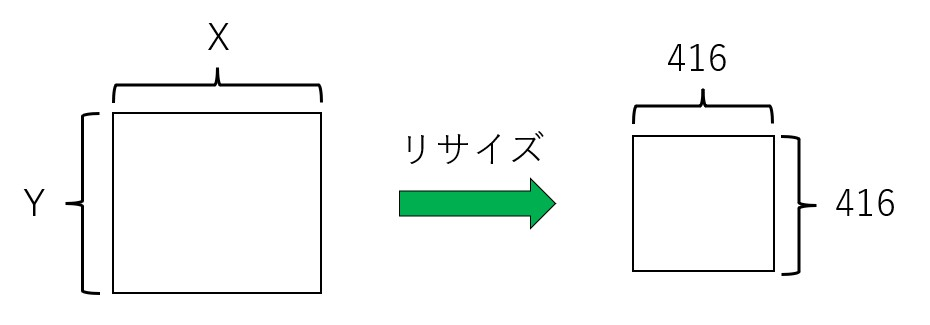
\includegraphics[scale = 0.8]{pict/pict5.jpg}
  \caption{リサイズ}
\end{figure}
図2.2にリサイズの工程を示した.
入力画像のサイズを横:X,縦:Yに対してリサイズ後のサイズは416pxの正方形である.

%次に正規化について示す.正規化とは特徴量の値の範囲を一定の範囲内に収めるように変換する処理のことである.
%\begin{equation}
%  \begin{split}
%  &x_{norm} = \frac{x-x_{min}}{x_{max}-x_{min}} \\
%  (x_{norm}:xを正規化&した値, x_{min}:xの最小値,x_{max}:xの最大値) \\
%  \end{split}
%\end{equation}
%式2.1ではある特徴量xに対して特徴量の取り得る最小値を引き,その値を
%特徴量の最大値と最小値の差つまり特徴量の取り得る範囲で割ることで
%正規化を行っている.これは特徴量の値を0から1の値に変換する処理であることから
%0,1スケーリングと呼ばれる.

\subsection{OpenCV}
OpenCVとはOpen Source Computer Vision Libraryの略称で,Intelが開発した画像・動画に関する処理機能をまとめた
オープンソースのライブラリである.OpenCVの持つ機能\cite{OpenCV}を以下に列挙する.
\begin{quote}
  \begin{itemize}
    \item 画像の入出力
    \item 画像の前処理
    \item 画像内のオブジェクト検出
    \item 画像への描写処理
    \item Deep Learning
  \end{itemize}
\end{quote}

\section{FPGA}
\subsection{FPGA概要}
FPGAはField Programmable Gate Arrayの略称であり,日本語に直訳すると「現場で構成可能なゲートアレイ」となる.
ここで,FPGA上には論理ゲートやトランジスタなどのハードウェアの構成に必要なパーツが搭載されている.
それらのパーツを必要に応じて配線で繋ぎ合わせることで専用ハードウェアを構成することができる.
このような専用ハードウェアの設計手法を「ゲートアレイ」と呼ぶ.
また,FPGAの他にも専用ハードウェアを設計することのできるデバイスとしてASIC(Application Specific Integrated Circuit)がある.
しかしこちらのASICでは,一度製造してしまったハードウェアは,製造後にその構成を変更することができない.
一方でFPGAは「現場で構成可能」という表現からもわかる通り,何度でもその構成を組み直すことが可能である.
以上より,FPGAは,日々最適化されていくシステムの中で,そのハードウェア構成を常に更新し続けられる点から高い柔軟性を持っている.

\subsection{Ultra96v2}
本研究で扱うFPGAボード.Ultra96v2に搭載されているZynq UltraScale+ MPSoC\cite{boardinfo}は,プロセッサとFPGAを
1チップに搭載しており,機能を以下に述べる.
%引用https://www.avnet.com/wps/portal/japan/products/product-highlights/ultra96/
\begin{quote}
  \begin{itemize}
    \item 高性能かつ大容量プログラムロジックを利用した高帯域な信号・画像処理
    \item Cortex-A53アプリケーションプロセッサで余裕のあるシステム(OS/GUI)プロセス処理実行
    \item Cortex-R5でタイミングクリティカルなリアルタイム処理をプログラムロジックと連携処理
  \end{itemize}
\end{quote}
以上の機能を持つことからも,自動車,医療,製造業,放送,通信などの幅広い分野で利用されている.

\section{ハードウェアアクセラレーション}
ここでは,ハードウェアアクセラレーション\cite{HWAccel}の概要を示す.
CPU(PS:Processing System)は複雑な制御に優れているが,膨大なデータ処理を必要とするアプリケーションには最適とは限らない.
こうした課題を抱えているアプリケーションに対して,アプリケーション内の大量の演算処理が必要な部分を切り離し,その処理のために
構成した専用ハードウェア(PL:Programmable Logic)で処理を行うことで高速化を図る手法のことをハードウェアアクセラレーションと呼ぶ.

本研究では,物体検出における前処理に対してハードウェアアクセラレーションをすることで,処理の高速化を図る.
%
%========エッジAIプラットフォーム開発=================================================================
\chapter{エッジAIプラットフォーム開発}
本章ではハードウェアアクセラレーションアプリケーション開発を円滑に進めるためのプラットフォームについて述べる.
\section{Vitis プラットフォーム概要}
Vitis プラットフォーム\cite{VitisPlatform}は,FPGAボード上で動作するハードウェアやソフトウェアの基となるアーキテクチャを定義する.
このVitis プラットフォームはFPGA上でPL(Programmable Logic)を用いて動作するアプリケーションのために作成する.
また,一つのVitis プラットフォーム上で複数のアプリケーションを作成することが可能である.
そのため,FPGAのハードウェア構成やOSの起動イメージを一から作成する必要が無くなる.

本研究では,アプリケーション開発を円滑に進めるためにVitis プラットフォームを作成し,そのプラットフォーム上で画像処理用アプリケーションを
作成する.

%\begin{quote}
%  \begin{itemize}
%    \item プラットフォームの再利用性:同じプラットフォーム上で異なるアクセラレーションアプリケーションを入れ替え可能
%    \item アプリケーションの移植性:最小限の操作で異なるプラットフォーム間でアプリケーションを移植可能
%    \item シミュレーション時間:カーネルを使用する協調シミュレーションの高速化
%    \item ランタイム:オープンソースのランタイムを使用してPCle®インターフェイスまたはエンベデッドインターフェイス経由でホストとデバイス間の通信を制御
%    \item システムデバッグ:システム全体の協調シミュレーションによって,全ハードウェアコンパイル時間を短縮
%  \end{itemize}
%\end{quote}
\section{Vitis プラットフォーム開発環境とツール}
ここではVitis プラットフォーム開発のための環境および使用するツールについて述べる.
\begin{quote}
  \begin{itemize}
    \item Ubuntu18.04.3 LTS・・・
    開発用PCのOSはUbuntuを用いた.開発ツールであるVivado,PetaLinux,Vitisのバージョンに対応させてUbuntuのバージョンは
    18.04を採用している.
    \item Vivado-v2019.2・・・
    Xilinx社が提供するハードウェア設計ツール.
    \item PetaLinux-v2019.2・・・
    Xilinx社がYocto ProjectをベースとしてZynqシリーズ用にカスタマイズしたLinuxディストリビューションの構築を行うためのフレームワーク.
    組み込みシステム向けLinuxをカスタマイズ,ビルド,およびデプロイするために必要なモノを全て提供する.
    本研究で用いるUltra96v2ボードに搭載されているZynq UltraScale+ MPSoCを含める多くのデバイスに対してLinuxシステムの開発を容易にする.
    \item Vitis-v2019.2・・・
    Xilinx社が提供するVitis統合ソフトウェアプラットフォーム.
    FPGA開発で用いるプラットフォームおよびアプリケーションの作成が可能.
  \end{itemize}
\end{quote}

\section{Vitis プラットフォーム作成}
ここでは,FPGAボードで実行するアプリケーション開発の基盤となるVitis プラットフォームの作成手順について述べる.
\begin{figure}[H]
  \center
  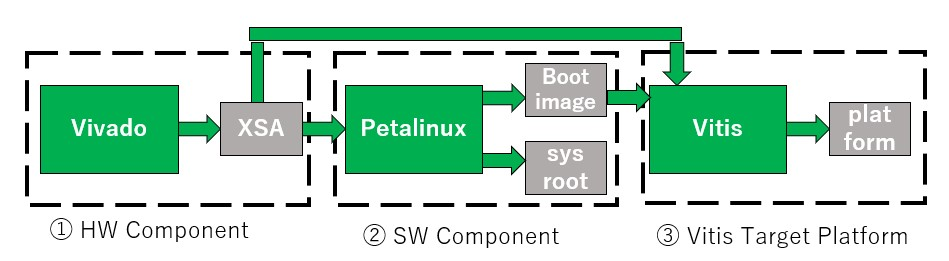
\includegraphics[scale = 0.8]{pict/pict7.jpg}
  \caption{Vitis プラットフォーム作成フロー}
\end{figure}
図3.1はプラットフォーム作成フローを示している.
はじめにVivadoを用いてハードウェアの構成を行い,XSAファイルとして出力する.この工程をHW(Hardware) Componentとする.
Ultra96v2上でLinuxOSを起動するためのファイル群をBoot image,ヘッダやライブラリが格納されている
rootディレクトリをsysrootと表す.Petalinuxを用いてこれらを作成する工程をSW(Software) Componentとする.
最後にHW ComponentとSW Componentの成果物をVitisで読み込みまとめることでVitis プラットフォームを作成する.この工程をVitis Target Platformとする.
ここで示した開発フローを,Xilinx提供のユーザガイド\cite{Xilinx-platform}を参考にして実行する.

\subsection{HW(Hardware) Component}
ここではハードウェアの構成を行う.
Vivadoを起動し,プロジェクト名をu96v2とした.

はじめに,BlockDesignと呼ばれる回路の設計を行う.
図3.2に作成したBlockDesignを示す.
\begin{figure}[H]
  \center
  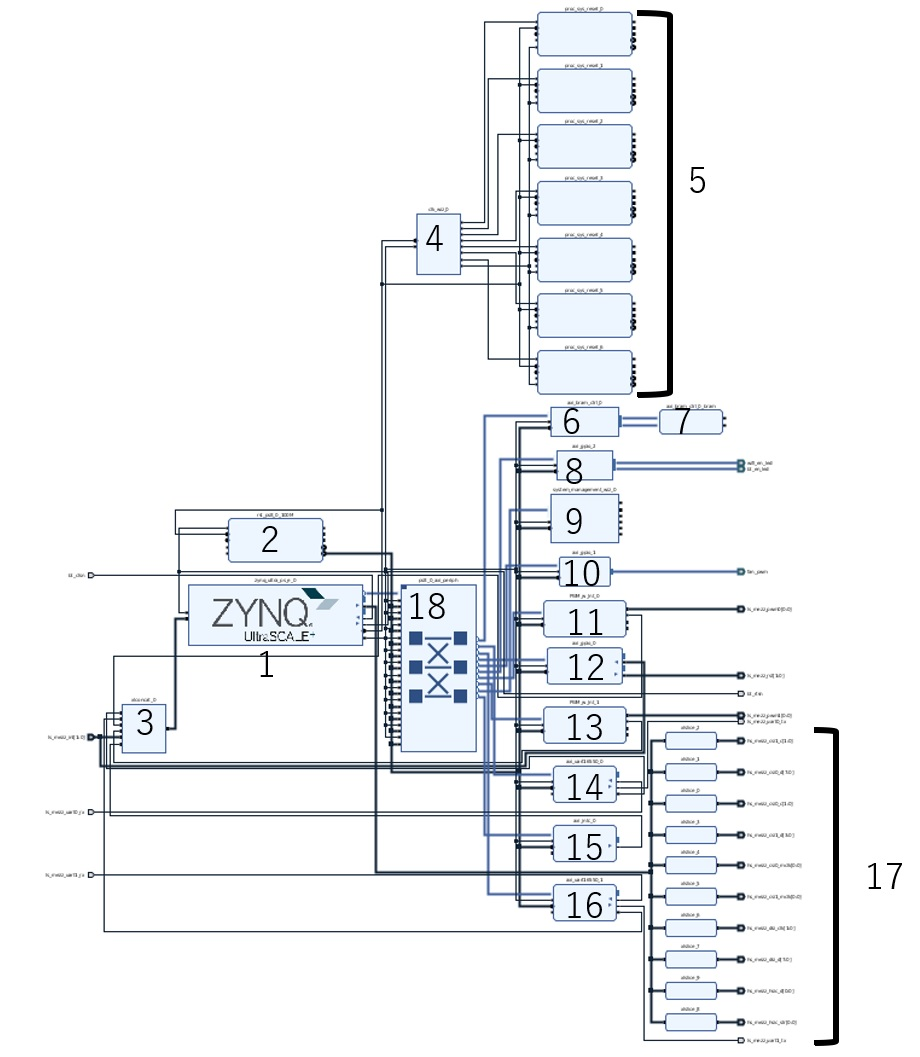
\includegraphics[scale = 0.4]{pict/pict2.jpg}
  \caption{HW BlockDesign}
\end{figure}
図3.2中の配線によって繋がれているブロックの部分をIP(Intellectual Property)
と呼び,このブロックは既に設計された回路モジュールを表している.
Ultra96v2ボードにはZynq UltraScale+ MPSoCと呼ばれるIPが搭載されている.
このIPはPS(Processing System)とPL(Programmable Logic)の部分に分かれており,
他のIPに対してクロックとリセットの供給を行う.作成したBlockDesignでは,
Zynq UltraScale+ MPSoCの出力クロックと出力リセットをClking Wizardに供給する.
Clocking WizardはPL部分にクロックの供給を行い,その出力周波数を指定することができる.
Clocking Wizardのクロック出力数はProcessor System Resetの数に合わせて5つに指定する.
またProcessor System Resetへのリセット入力はZynq UltraScale+ MPSoCの出力リセットから供給する.
図3.2に示したBlockDesignにおけるIPの種類,IPの名称,IPの入出力についてを表3.1に示す.
\begin{table}[H]
  \caption{BlockDesignにおけるIP}
  \label{table:SpeedOfLight}
  \centering
   \begin{tabular}{llll}
    \hline
    IP種類 & IP名称 & 入力 & 出力 \\
    \hline \hline
    Zynq UltraScale+ MPSoC & zynq_ultra_ps_e_0 & dout[0:0] & pl_resetn0 \\
    & & & pl_clk0 \\
    \hline
    Concat & xlconcat_0 & & dout[0:0] \\
    \hline
    Clocking Wizard & clk_wiz_0 & pl_resetn0 & clk_out1 \\
    & & pl_clk0 & clk_out2 \\
    & & & clk_out3 \\
    & & & clk_out4 \\
    & & & clk_out5 \\
    & & & locked \\
    \hline
    Processor System Reset & proc_sys_reset_0 & clk_out1 & \\
    & & locked & \\
    & & pl_resetn0 & \\
    \hline
    Processor System Reset & proc_sys_reset_1 & clk_out2 & \\
    & & locked & \\
    & & pl_resetn0 & \\
    \hline
    Processor System Reset & proc_sys_reset_2 & clk_out3 & \\
    & & locked & \\
    & & pl_resetn0 & \\
    \hline
    Processor System Reset & proc_sys_reset_3 & clk_out4 & \\
    & & locked & \\
    & & pl_resetn0 & \\
    \hline
    Processor System Reset & proc_sys_reset_4 & clk_out5 & \\
    & & locked & \\
    & & pl_resetn0 & \\
  \hline
  \end{tabular}
\end{table}
FPGAではFPGA内部のロジックに供給するクロックを指定する必要がある.
その機能を有しているIPが図3.2中のClocking Wizardであり,
実際に出力されるクロックの詳細について表3.2に示す.
\begin{table}[H]
  \caption{Clocking Wizardによる出力クロック}
  \label{physics}
  \centering
  \begin{tabular}{ccc}
    \hline
    ポート名 & \multicolumn{2}{c}{出力周波数 (MHz)} \\
    \cmidrule(lr){2-3}
     & 要求 & 実際 \\
    \hline
    clock_out1 & 100 & 100 \\
    clock_out2 & 200 & 200 \\
    clock_out3 & 300 & 300 \\
    clock_out4 & 400 & 400 \\
    clock_out5 & 600 & 600 \\
    \hline
    \end{tabular}
\end{table}
以上のBlockDesignの作成を終了し,u96v2.xsaというファイル名で保存することでここでの工程は終了する.

\subsection{SW(Software) Component}
この工程ではPetalinuxを用いて作業を行う.Petalinuxの保持しているツールの中で本研究で用いるのは,
petalinux-create,petalinux-config,petalinux-buildである.
SW Componentを作成する手順について図3.3に示す.
\begin{figure}[H]
  \center
  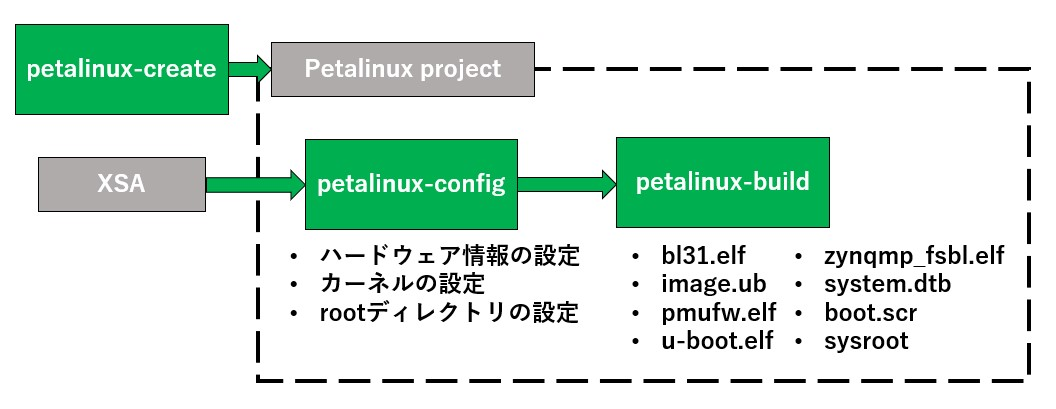
\includegraphics[scale = 0.8]{pict/pict9.jpg}
  \caption{SW Component作成フロー}
\end{figure}

はじめに,プロジェクト名をu96v2としてpetalinux projectの専用ディレクトリを作成する.プロジェクトの作成には
petalinux-createツールを使用する.petalinux project内でなければPetalinuxの保持するツールが利用できないため,
以降はこのディレクトリ内でSW Componentの工程を行う.

作成したディレクトリに移動し,petalinux-configツールを用いてu96v2.xsaからハードウェアコンポーネントの情報の
アップデート,Linuxカーネルの設定,rootディレクトリの設定の順で行う.

はじめに,ハードウェア情報のアップデートにおける作業を述べる.
Ultra96v2を起動するには,起動用データをSDカードに格納し,それをUltra96v2に挿入することで起動させる.
ここで,rootディレクトリとしてSDカードに格納されるファイルはEXT型である必要があるため,Root filesystem typeを
EXTに設定する.
次に,PetalinuxのベースはYocto Projectであるため,Yoctoの設定でデバッグを有効にする.
最後にUARTの設定を行う.Ultra96v2はシリアル通信における標準入出力をUART1で行うため,psu_uart_1を指定する.
以上の変更を保存してハードウェア情報のアップデートは終了する.

次にLinuxカーネルの設定について述べる.ここではデバイスドライバのサイズをデフォルト値が254MBだったため1024MBに変更した.

加えて,Petalinuxプロジェクトの中にuser-rootfsconfigというファイルがある.これはrootファイルシステムに含めるパッケージを管理する.
ここで,ホストとアクセラレータの通信を容易にするソフトウェアインターフェイスであるXRT(Xilinx Runtime Library),
Linuxカーネルドライバであるzocl,複数の異なる計算用リソースを併用するために用いるOpenCL,画像処理ライブラリであるOpenCVの項目をuser-rootfsconfigに追加する.
ここで追加したzoclドライバをデバイスツリーに含める必要がある.デバイスツリーはsystem-user.dtsiというファイルに記述されているため,このファイルを編集して
zoclを追加した.

最後にrootディレクトリの設定を行う.ここでは作成したアプリケーションを動かすために必要となるライブラリを有効にする.
具体的にはgccランタイムのC++,Python3,OpenCV,user packageを有効にする.
以上でPetalinux-configツールを用いた設定を終了する.

最後に,設定したPetaLinuxプロジェクトの内容を参照してUltra96v2上で動作するLinuxOSの起動イメージおよびsysrootの生成を行う.
この作業はpetalinux-buildツールを用いる.ここでは複数のファイルが生成されるが,その中にsdk.shというファイルがある.
これは自己解凍ファイルであり,このファイルを実行し,自己解凍することでsysrootディレクトリが生成される.
ここまで,LinuxOSを起動するためのコンポーネントを作成してきた.これらのコンポーネント構造をまとめるファイルが必要である.
そのファイル名をlinux.bifとして作成する.
以下にSW Componentにおける成果物のうち,後のVitis Target Platformの作成で用いるファイルおよびディレクトリを列挙する.
\begin{quote}
  \begin{itemize}
    \item bl31.elf
    \item image.ub
    \item pmufw.elf
    \item u-boot.elf
    \item zynqmp_fsbl.elf
    \item system.dtb
    \item boot.scr
    \item linux.bif
    \item sysroot
  \end{itemize}
\end{quote}
新たにbootという名前のディレクトリを作成し,上記の生成物の内,
bl31.elf,image.ub,pmufw.elf,u-boot.elf,zynqmp_fsbl.elf,system.dtb,boot.scrを格納してまとめて管理する.

\subsection{Vitis Target Platform}
HW ComponentとSW Componentの工程で得られた成果物とVitisツールを用いて
Vitis Target Platformの作成を行う.設定項目と設定内容を表\ref{vtpset}に示す.
\begin{table}[H]
  \caption{Vitis Target Platform初期設定}
  \label{vtpset}
  \centering
  \begin{tabular}{ll}
    \hline
    項目 & 内容 \\
    \hline
    XSA_file & u96v2.xsa\\
    OS & Linux \\
    Processor & psu_cortexa53\\
    Bif file & linux.bif \\
    Boot Component Directory & boot \\
    Linux Image Directory & boot \\
    Sysroot Directory & sysroot/aarch64-xilinx-linux \\
    \hline
    \end{tabular}
\end{table}
表\ref{vtpset}の設定内容について記述する.
Vitisを起動後,HW Componentで示したXSAファイルを選択して,
Platform Projectを作成する.Domein設定を開き,OSをLinux,Processorをpsu_cortexa53に指定する.
加えてBifファイルをlinux.bif,Boot Components DirectoryおよびLinux Image DirectoryをSW Componentの
工程でまとめたbootディレクトリ,Sysroot Directoryにsysroots/aarch64-xilinx-linuxディレクトリを指定した.
以上の設定後,Vitisツール上でビルドボタンを押すことで,設定内容をまとめてVitis Target Platformとして出力される.
ここで作成したプラットフォームが格納されているディレクトリ名をu96v2_pfmとした.
ここで作成したVitis Target Platformを用いて第4章のアプリケーション開発を行う.

\section{Vitis Vision Library}
FPGA用の画像データ前処理アプリケーションはVitisというツールで作成するため,Vitisツール専用のライブラリを用いる必要がある.
Vitisを用いたFPGAアプリケーション開発に対してXilinx社が提供しているライブラリにVitis アクセラレーションライブラリがある.
このライブラリの一種で,画像処理に対する機能を含んだものがVitis Vision Libraryであり,OpenCVの画像処理関数の多くを含んでいる.

%Vitis Vision Libraryの特徴を以下に列挙する.
%\begin{quote}
%  \begin{itemize}
%    \item 色およびビット深度変換,ピクセルごとの算術演算,幾何変換,統計,フィルター,特徴検出,分類,3D再構成など性能に最適化された機能の提供
%    \item カラー画像処理のネイティブサポート,マルチチャネルストリーミングのサポート
%    \item オンチップメモリまたは外部メモリ間のデータ移動を効率的に管理して最大限の性能を達成
%    \item ビジョンパイプラインに求められる演算能力をすばやく評価して最適なデバイスを選択
%    \item ビジョンおよび画像処理アルゴリズムを高速化する方法を示すサンプルデザインを提供
%    \item 関数パラメータを活用し,1クロックサイクルで複数ピクセルを処理してスループット要件を満たす
%  \end{itemize}
%\end{quote}
%
%========アプリケーションの実装=================================================================
\chapter{アプリケーションの実装}
本章では物体検出における画像前処理アプリケーションの作成について述べる.
Ultra96v2のようなFPGAボードには基本的なシステム全体の制御を行うPS(Processing System)部分と
特定の演算処理などに用いられるPL(Programmable Logic)部分が存在する.
本研究では,PSのみを利用して処理を行うアプリケーションと
PSに加えてPLを用いて処理を行うアプリケーションの作成を行う.
\section{アプリケーション作成(PS)}
実行時にPS(Processing System)のみを用いて画像の前処理を行うアプリケーションの作成について述べる.
このアプリケーションのソースコードはPythonで記述しており,
ファイル名をprepro_PS.pyとし以下に示す.
\begin{lstlisting}[caption=prepro_PS.py]
  import glob
  import sys
  import time
  import cv2
  import numpy as np
  
  re_length = 416
  total = 0
  
  for i in range(600):
  
      img = cv2.imread("./mask_before/Mask_" + str(i+1) + ".jpg")
  
      time_sta = time.time()
  
      h, w = img.shape[:2]
  
      re_h = re_w = re_length/max(h,w)
  
      img_resize = cv2.resize(img, dsize=None, fx=re_h, fy=re_w)
  
      time_end = time.time()
      t = time_end - time_sta
      total = total + t
  
  print("time:" + str(total) + "[ms]")
\end{lstlisting}
prepro_PS.pyの概要を以下に述べる.
1行目から5行目までは必要なモジュールを利用するための記述である.
7行目の変数re_lengthは入力画像に対してリサイズした後の画像サイズ
である416pxを定義している.ここでは入力画像の長辺を416pxにリサイズ
することを想定しており,リサイズ後も長辺と短辺の大きさの比率は変わらない.
10行目から20行目までの画像処理の部分の説明をする.
前処理を行うサンプル画像の枚数は600枚で行ったので10行目のrangeの中は
600に指定している.12行目ではopencvを利用した入力画像の取得を行っており,
続けて16行目で入力画像の縦のサイズ:h,横のサイズ:wを取得している.
18行目では入力画像を変換する倍率の計算を行っており,リサイズ後の長辺サイズである
416pxを入力画像の縦,横のピクセルサイズのうち大きい方で除算することにより倍率を計算している.
20行目のimg_resizeには入力画像をリサイズした後の配列を格納する.
opencvの関数であるcv2.resizeに対して入力画像imgと18行目で計算した倍率である
re_hとre_wを引数として渡すことでリサイズ処理を行う.

リサイズにかかる処理時間は,変数totalに格納する.リサイズの処理を行う前後で
時刻を取得し,その処理時間の計算を行う.1枚当たりにかかった処理時間を変数totalに
加算していくことで,最終的に600枚当たりの処理時間の計測を行っている.

\section{アプリケーション作成(PS+PL)}
PS(Processing System)に加えてPL(Programmable Logic)を用いるアプリケーションの作成は,3章で作成したVitis Target Platformである
u96v2_pfmを利用して行う.
Vitisツールを起動し,プラットフォームをu96v2_pfmに指定した.
その後サンプルからVitis Vision Libraryを選択する.Vitis Vision LibraryはOpenCVの機能の一部を有しており,
それをVitisツールで利用できる形にカスタマイズされたライブラリである.
そのライブラリの中からresizeを選択する.作成したプログラムを以下に示す.

※完成したら書きます

%
%========ここにC++で記述されたリサイズのソースコードを貼る.
%
%========ここにソースコードの説明
%
%========評価実験=======================================================================
\chapter{評価実験}
本章ではこれまでに作成してきたアプリケーションの実行するまでの実験準備,実行手順,実験結果について述べる.
\section{実験準備}
ここではUltra96v2を起動する前に行う必要のある準備をデータセット,SD_Cardの作成の順に述べる.
\subsection{データセット}
実験に用いるサンプル画像は,Vitis-AIのUltra96v2上動作に関する記事\cite{SamplePictWeb}に記載されている
マスクを着用している人々の画像データセットであるMask Dataset\cite{SamplePictDrive}を利用した.
このデータセットの内,600枚の画像に対して前処理プログラムを実行する.サンプル画像の例を図5.1に示す.
\begin{figure}[H]
  \center
  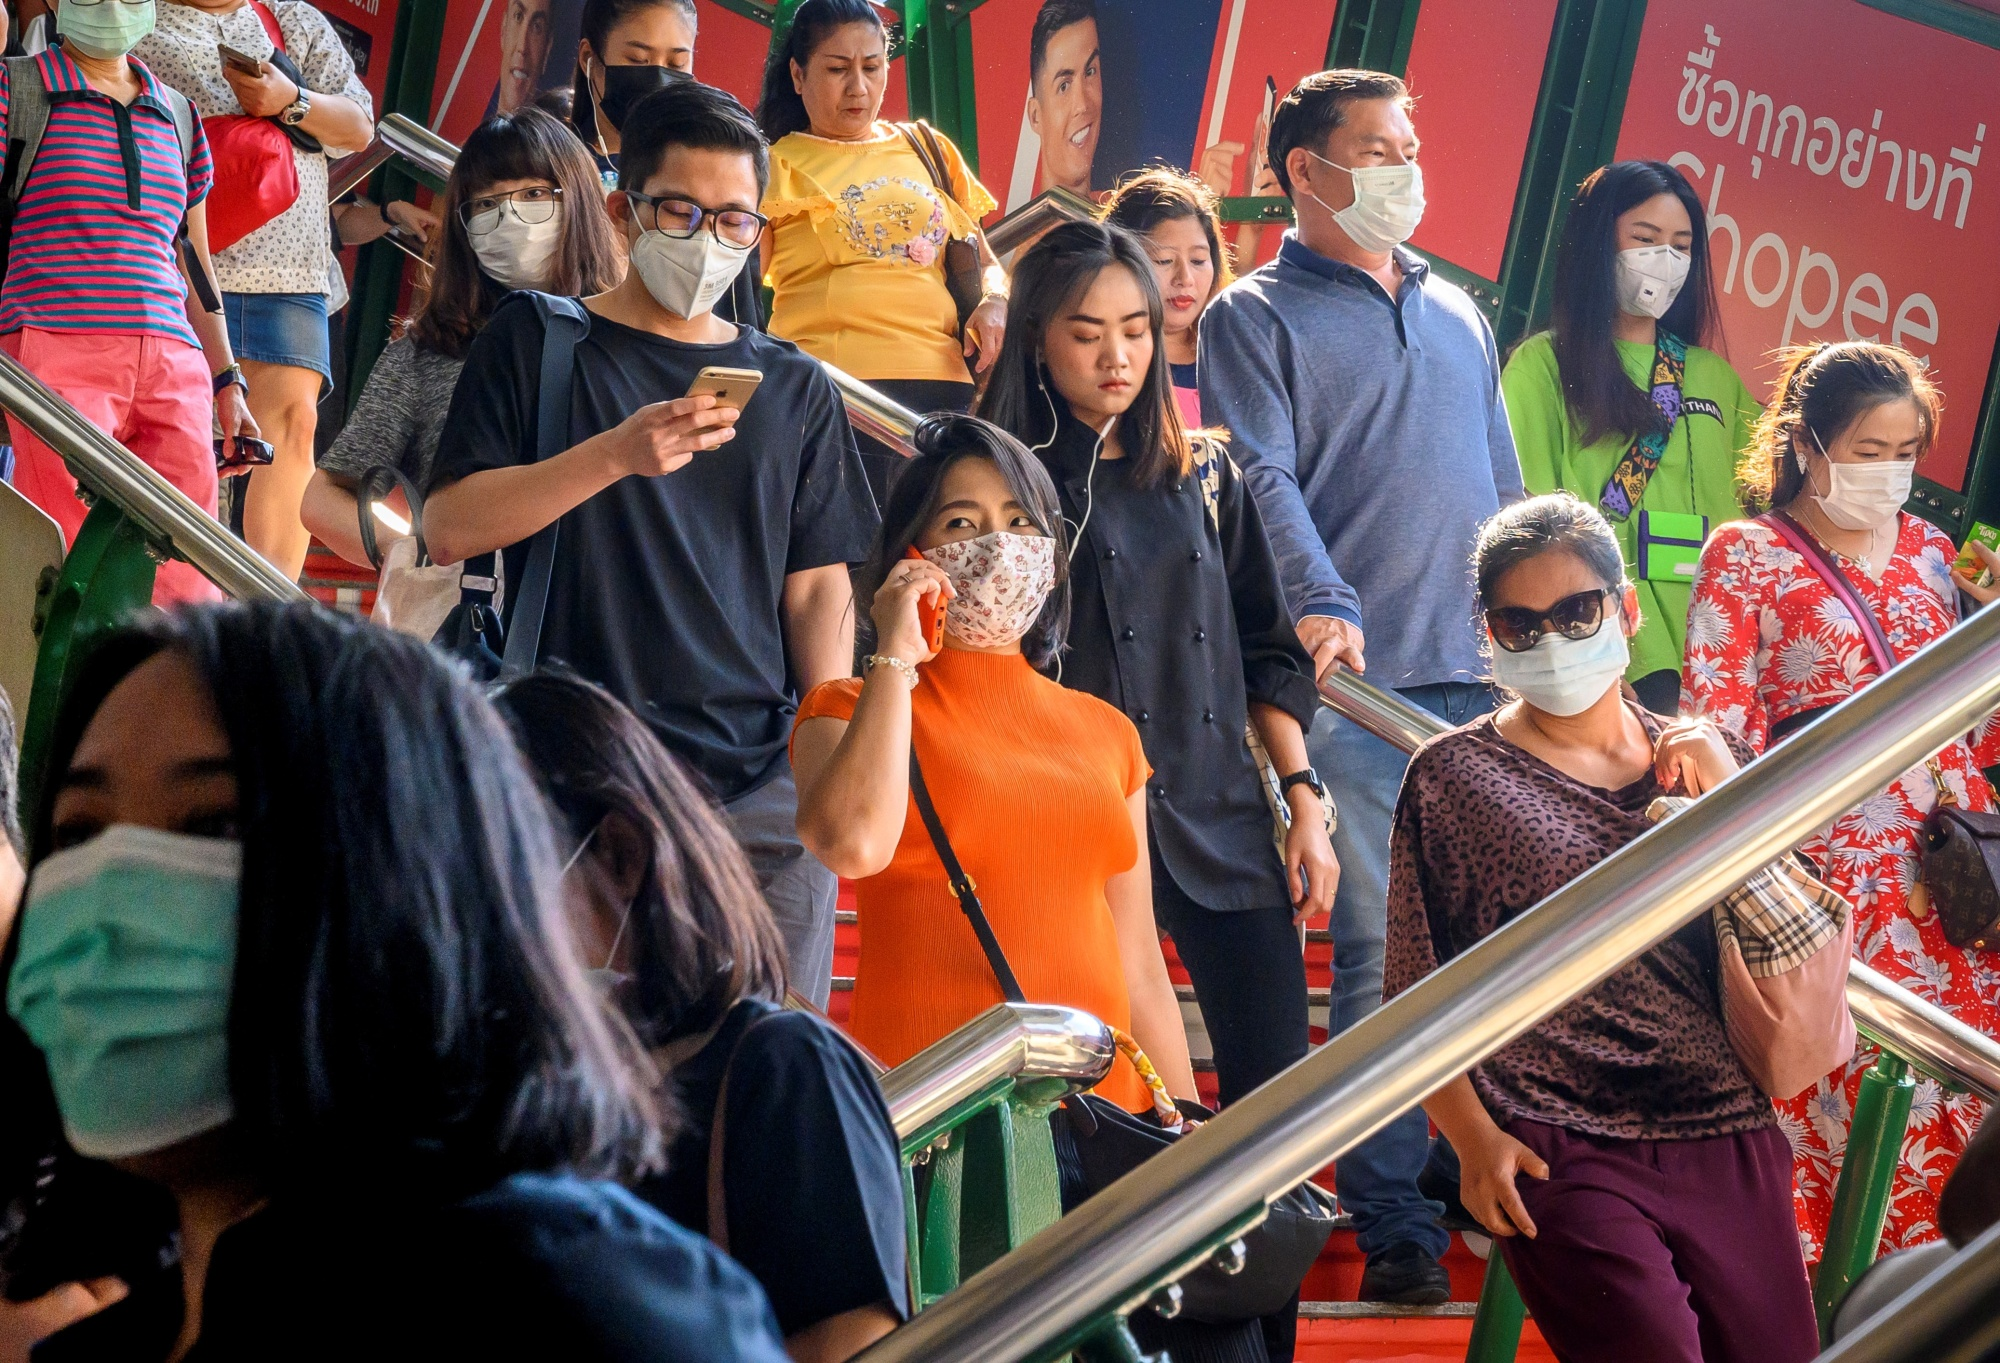
\includegraphics[scale = 0.17]{pict/Mask_1.jpg}
  \caption{Mask Dataset Sample Picture}
\end{figure}

\subsection{SD_Cardの作成}
Ultra96v2はOSの起動イメージとrootディレクトリを一つのSDカード内の異なるパーティションに格納する必要がある.
そのため,MicroSDカードを2つのパーティションに分割する.分割の概要について表\ref{SDpartition}に示す.
\begin{table}[H]
  \caption{MicroSDのパーティション分割}
  \label{SDpartition}
  \centering
  \begin{tabular}{|c|l|l|}
    \hline
    項目 & 第1パーティション & 第2パーティション \\
    \hline \hline
    名称 & boot & rootfs \\
    ファイルシステム & FAT32 & ext4 \\
    サイズ & 4GB & 28GB \\
    \hline
    \end{tabular}
\end{table}
表\ref{SDpartition}のように,第1パーティションの名称をboot,ファイルシステムはFAT32,サイズは4GBに指定した.
続いて,第2パーティションの名称はrootfs,ファイルシステムはext4,サイズは28GBに指定した.
名称はそれぞれの格納するファイルを表している.
また,Ultra96v2にはZynq UltraScale+ MPSoCと呼ばれるデバイスが搭載されている.このデバイスはFATファイルシステムにある起動用ファイル
を呼び出すことで起動する.
サイズは,格納するファイルのサイズに合わせて指定してある.
次に,作成したデータの書き込みについて図5.2に示す.
\begin{figure}[H]
  \center
  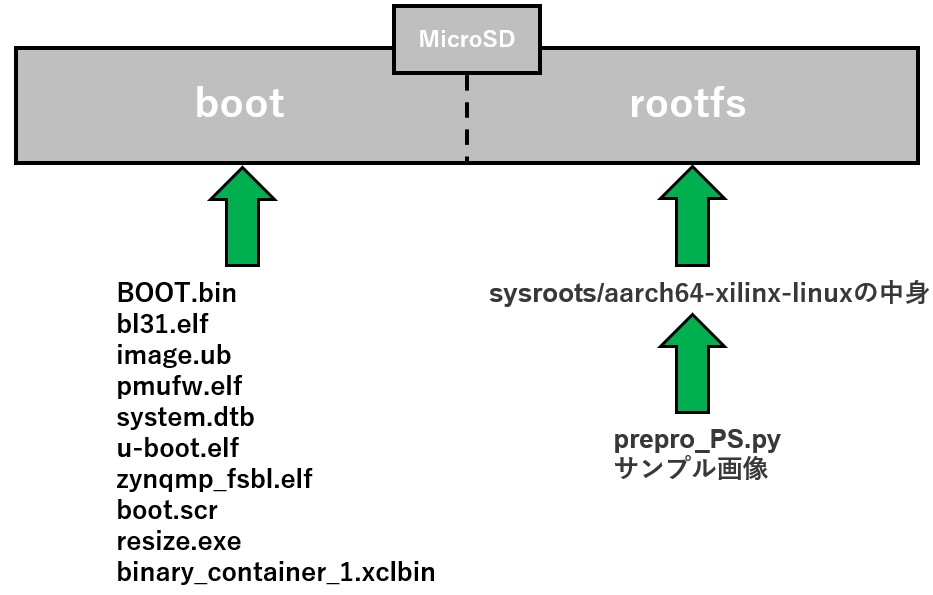
\includegraphics[scale = 0.7]{pict/pict8.jpg}
  \caption{SDカードへのデータ格納}
\end{figure}
第1パーティションであるbootには図5.2に示している10種類ののファイルを書き込む.
第2パーティションであるrootfsにはLinuxシステムのrootファイルを書き込む.
同時に,作成したUltra96v2上のデバイスのうち,PS(Processing System)のみで処理を行う画像処理
アプリケーションと実験に用いるサンプル画像のデータセットもこの第2パーティションに書き込む.

\subsection{実験環境の構築}
ここではUltra96v2を起動し,これまで作成してきたアプリケーションを実行する前にやっておく必要のある環境構築について述べる.

必要なファイルの書き込みが完了したので,MicroSDカードをUltra96v2に挿入し,PCとシリアル通信を行う.
シリアル通信用ツールであるgtktermを起動し,設定画面を開き,ポートを/dev/ttyUSB1に,ボーレートを115200に指定した.
Ultra96v2の起動ボタンを押すと,Linuxカーネルが起動する.
最初に,Ultra96v2のWi-Fi設定を行う.設定が完了したら.PS(Processing System)のみを用いて画像処理を行うアプリケーションのために,
Python用のOpenCVをダウンロードする.Python3でcv2をインポートできることを確認した.

\section{アプリケーションの実行}
ここでは作成したアプリケーションを実際にUltra96v2上で実行した手順について述べる.
\subsection{アプリケーションの実行(PS)}
作成したPS(Processing System)のみを用いて画像処理を行うアプリケーションを実行する.
画像処理アプリケーションであるprepro_PS.pyとサンプル画像が格納されているmask_beforeディレクトリのあるディレクトリで以下のコマンドを実行した.

python3 prepro_PS.py

\subsection{アプリケーションの実行(PS+PL)}
※実行したら書きます.

\section{実験結果}
※結果出たら書きます.
%
%========考察========================================================================
\chapter{考察}
本章では,ハードウェア実装した前処理の性能に対する考察と,本研究の今後の展望についての考察を述べる.

まず,ハードウェア実装した前処理の性能に対する考察を述べる.
※実験終わったら書きます

次に,本研究の今後の展望について考察を述べる.本研究では,物体検出における前処理の部分の中でも,
特にリサイズの処理に対して焦点を当てた.しかし実際の前処理では,リサイズだけの処理をするわけではなく,
正規化などの他の処理も行う,この前処理は推論モデルによってまちまちである.そのため,リサイズ以外の前処理についても
ハードウェア実装をすることで高速化できると考える.
また,エッジコンピューティングにおける速度以外の課題であるリソースの使用率や消費電力の項目についてもハードウェア化することで
どのような変化をもたらすか検証する必要がある.
加えて,ハードウェア実装した前処理を,物体検出に組み込み,前処理から推論処理までの物体検出全体の処理速度にどの程度影響を
及ぼすのかも検証する必要がある.
%=======あとがき=====================================================================
\chapter{あとがき}
本研究では,物体検出におけるリアルタイム性を課題として取り上げ,前処理を高速化することを目的とした.
この目的を成し遂げるため,前処理の部分をハードウェア実装することを目標とした.
本研究を進めるにあたって,はじめに開発ツールであるVivado,Petalinux,Vitisの使用方法について学習を行った.
その後,プラットフォームの作成,アプリケーションの作成,FPGAボードでの実験,性能評価の順で実行した.

本研究の結果
※実験終わったら書きます

しかし,ハードウェア実装できた物体検出における画像処理はリサイズ処理のみであり,さらに高速化を図るためには,その他の前処理についても
ハードウェア実装する必要がある.加えてエッジデバイスにおけるリアルタイム性以外の課題であるリソース使用率や消費電力については
検証できていないのため,これらの項目についても検証する必要がある.

以上を今後の課題とし,解決することでエッジデバイスにおける物体検出のリアルタイム性向上につながると考える.

%=====================================================================================
\chapter*{謝辞} %章を付けずにタイトル表示
\addcontentsline{toc}{chapter}{謝辞} %章立てせずに目次に追加するおまじない
本研究,論文作成を進めるにあたり,御懇篤な御指導,御鞭撻を賜りました本学高橋寛教授ならびに
甲斐博准教授,王森レイ講師に深く御礼申し上げます.

また,審査頂いた本学甲斐博准教授,遠藤慶一准教授ならびに宇戸寿幸准教授に深く御礼申し上げます.

最後に,多大な御協力と貴重な御助言を頂いた計算機/ソフトウェアシステム研究室の諸氏に厚く御礼申し上げます.
%=====================================================================================
%\chapter*{参考文献}
\addcontentsline{toc}{chapter}{参考文献} %章立てせずに目次に追加するおまじない
\renewcommand{\bibname}{参考文献} %これがないと,タイトルが「関連図書」になってしまう
\bibliography{bibtexファイル名} %bibtexファイルの読み込み
\bibliographystyle{junsrt} %本文に\cite{}を入れることで,参考文献表示
\begin{thebibliography}{99}
  \bibitem{AccelTemp} 小西祥之,国宗大介,西田芳隆,ミラクシアエッジテクノロジー株式会社, \\2021, \\"物体検出におけるエッジ環境での推論高速化と精度上昇", \\\url{https://www.jstage.jst.go.jp/article/pjsai/JSAI2021/0/JSAI2021_3I4GS7a02/_pdf/-char/ja}, \\(参照2023-01-19)
  \bibitem{OpenCV} ケイエイブル株式会社, \\"初めてのOpen CV(画像処理ライブラリ)ガイド" \\\url{https://www.klv.co.jp/corner/python-opencv-what-is-opencv.html}, \\(参照2023-01-19)
  \bibitem{boardinfo} AVNET, \\"Ultra96開発ボードでXilinx Zynq UltraScale+ MPSoCを手軽に評価", \\\url{https://www.avnet.com/wps/portal/japan/products/product-highlights/ultra96/}, \\(参照2023-01-19)
  \bibitem{HWAccel} Xilinx, \\"アクセラレーションコンピューティングとは何か.そしてなぜ必要なのか", \\\url{https://japan.xilinx.com/applications/adaptive-computing/what-is-accelerated-computing-and-why-is-it-important.html}, \\(参照2023-01-29)
  \bibitem{VitisPlatform} Xilinx, \\"Vitis 統合ソフトウェアプラットフォーム,プラットフォームベースフロー", \\\url{https://japan.xilinx.com/products/design-tools/vitis/vitis-platform.html}, \\(参照2023-01-19)
  \bibitem{Xilinx-platform} Xilinx, \\"Vitis 統合ソフトウェアプラットフォームの資料:エンベデッドソフトウェア開発", \\2020-06-24, \\\url{https://docs.xilinx.com/r/2020.1-日本語/ug1400-vitis-embedded}, \\(参照2023-01-18)
  \bibitem{SamplePictWeb} Qiita, \\"Vitis-AI v1.4 on Ultra96v2", \\2021-11-06, \\url{https://qiita.com/lp6m/items/4117a3bab185afedfd5f}, \\(参照2023-01-19)
  \bibitem{SamplePictDrive} Google Drive, \\"Mask_Dataset", \\2020-02-26, \\url{https://drive.google.com/drive/folders/1aAXDTl5kMPKAHE08WKGP2PifIdc21-ZG}, \\(参照2023-01-19)
\end{thebibliography}
\end{document}